\begin{tikzpicture} [overlay,remember picture]
       \draw [line width=0.5mm ] 
        ($ (current page.north west) + (1.2cm, -1.2cm) $)
        rectangle
        ($ (current page.south east) + (-1.2cm, 1.2cm) $);
\end{tikzpicture}
\thispagestyle{empty}

\hfill\textbf{WPS 2014-15/11}

\vfill

\begin{center}
    \textbf{EXPLORING THE BOUNDARY CONDITIONS OF THE RELATIONSHIP BETWEEN LMX AND WORK ENGAGEMENT}
\end{center}

\vfill

\begin{center}

    MOHD. HARIS MINAI\\
    Doctoral Student, Human Resource Management Group\\
    Indian Institute of Management Lucknow\\
    email: mhminai@iiml.ac.in\\

    \vspace{1\baselineskip}

    HEMANG JAUHARI\\
    Doctoral Student, Human Resource Management Group\\
    Indian Institute of Management Lucknow\\
    email: hemang.jauhari@iiml.ac.in\\

    \vspace{1\baselineskip}

    DR. SHAILENDRA SINGH\\
    Professor, Human Resource Management Group\\
    Indian Institute of Management Lucknow\\
    email: shail@iiml.ac.in\\

    \vspace{1cm}

\end{center}

\vfill

\begin{center}
    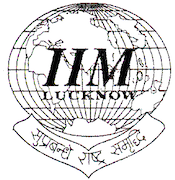
\includegraphics[width=2.5cm]{../config/iiml-logo}\\
    Indian Institute of Management\\
    Prabandh Nagar\\
    Off Sitapur Road\\
    Lucknow (U.P.)  -- 226013\\
\end{center}

\newpage

\vspace{\fill}

\begin{center}
\textbf{ABSTRACT}
\end{center}

Keeping employees engaged is increasingly becoming indispensable for organizations. Usually the first level leader of an employee is charged with maintaining an employee and getting work of high order through him. Given the limited attentional resources at the disposal of the manager, this is a challenging task.

In this study we study the effect of building a high quality relationship with a subordinate and its impact on subordinate work engagement. Given that exchanges in the organization happen in a context. We also explore the contextual role of personal and organizational moderators on this relationship.

We collect cross sectional data from 277 employees in the Indian IT industry. Analysis by way of hierarchical moderated regression shows that core self-evaluations negatively moderate the relationship between LMX and work engagement. On the other hand value congruence with the organization conceptualized as P--O Fit positively moderates this relationship.

Impact on theory, practice are discussed as well as avenues for future research.

\emph{\textbf{keywords:}} LMX, CSE, P--O Fit, leader-member exchange, core self-evaluations, person organization fit, value congruence, work engagement

\vfill

\newpage

\doublespacing

